\documentclass[12pt,a4paper,]{scrreprt}
\usepackage[ngerman]{babel}
\usepackage[onehalfspacing]{setspace}
\usepackage[utf8]{inputenc}
\usepackage{graphicx}
\usepackage{array}
\usepackage{gnuplottex}
\usepackage{siunitx}
\let\phi\varphi
\usepackage{multicol}
\usepackage{capt-of}
% * <henni.jaeger@gmail.com> 2016-11-09T12:56:56.224Z:
%
% ^.
\usepackage{amsmath}
\usepackage{ulem}
\usepackage{amsthm}

\setkomafont{chapter}{\fontsize{20bp}{22.2bp}\selectfont\bfseries}
\setkomafont{section}{\fontsize{14bp}{18.8bp}\selectfont\bfseries}
\setkomafont{subsection}{\fontsize{12bp}{14.4bp}\selectfont\bfseries}
\renewcommand{\chapterheadstartvskip}{\vspace*{-1\topskip}}
\renewcommand{\chapterheadendvskip}{\vspace*{0.5\topskip}}

%---------------------------------------------------------------------------------------------------------------------------------------------------------------
% Ende der Einstellungen
%---------------------------------------------------------------------------------------------------------------------------------------------------------------

%---------------------------------------------------------------------------------------------------------------------------------------------------------------
%Ab hier gibt es Inhalt
%---------------------------------------------------------------------------------------------------------------------------------------------------------------
\begin{document}

\title{Trägheitsmomente aus Drehschwingungen \\ (Zweitkorrektur)}
\author{Henrik Jäger \\ 3114168 \and Lena Majer \\ 3115808}
\subtitle{M10a \\  Assistent: Sascha Kolatschek}
\subject{Physikalisches Praktikum I}
\publishers{Universität Stuttgart}
%\thanks{Assistent: Sascha Kolatschek}
\date{10. Oktober 2016}
\maketitle% Titelei

\tableofcontents   %Inhaltsverzeichnis

\chapter{Einleitung}
		\section{Ziel}
			In dieser Aufgabe geht es um die Bestimmung eines Trägheitsellipsoids. Hierfür muss zunächst die Winkelrichtgröße der Schwenkfeder bestimmt werden.
		\section{Grundlagen}
			Die in diesem Versuch notwendigen Kenntnisse befassen zum großen Teil das Trägheits-moment. Das Drehmoment wird durch ein Integral über die Massenelemente und deren Abstand zur Drehachse bestimmt. \\
            \begin{equation}
            J = \int r^2 dm
            \end{equation}
			Ist bei einem festen Körper die Drehachse von einer Drehachse durch den Schwerpunkt verschoben, spielt der Steinersche Satz eine wichtige Rolle.  Hierfür gilt:\\
			\begin{equation}
				J=J_s + m \cdot r^2
			\end{equation}
Die Differentialgleichung einer Drehschwingung ohne Dämpfung ist gegeben durch:
\begin{equation}
J \cdot \frac{ d^2 \phi}{dt^2}=- D' \phi
\end{equation}
Hierbei entspricht D' der Winkelrichtgröße und $\phi$ dem Drehwinkel.
Die Schwingdauer, die durch die Lösung der Differentialgleichung (1.3) bestimmt wird, ist gegeben durch:
\begin{equation}
T(\omega)=2\pi \sqrt{\frac{J(\omega)}{D'}}
\end{equation}
Das Trägheitsmoment entspricht einem Tensor mit 9 Komponenten. Handelt es sich um ein Hauptträgheitssystem, so sind 3 Komponenten linear unabhängig. Andernfalls sind bei einem symmetrischen Tensor 6 der 9 Komponenten voneinander linear unabhängig.\\
Durch eine Hauptachsentransformation gelingt eine Darstellung der Form:
\begin{equation}
\frac{x^2}{a^2}+\frac{y^2}{b^2}+\frac{z^2}{c^2}=1
\end{equation}
Hierbei ist bereits zu erkennen, dass es sich um einen Ellipsoid handelt.
\pagebreak
            
	\chapter{Messprinzip mit Skizze und Versuchsablauf}
    \begin{center}
    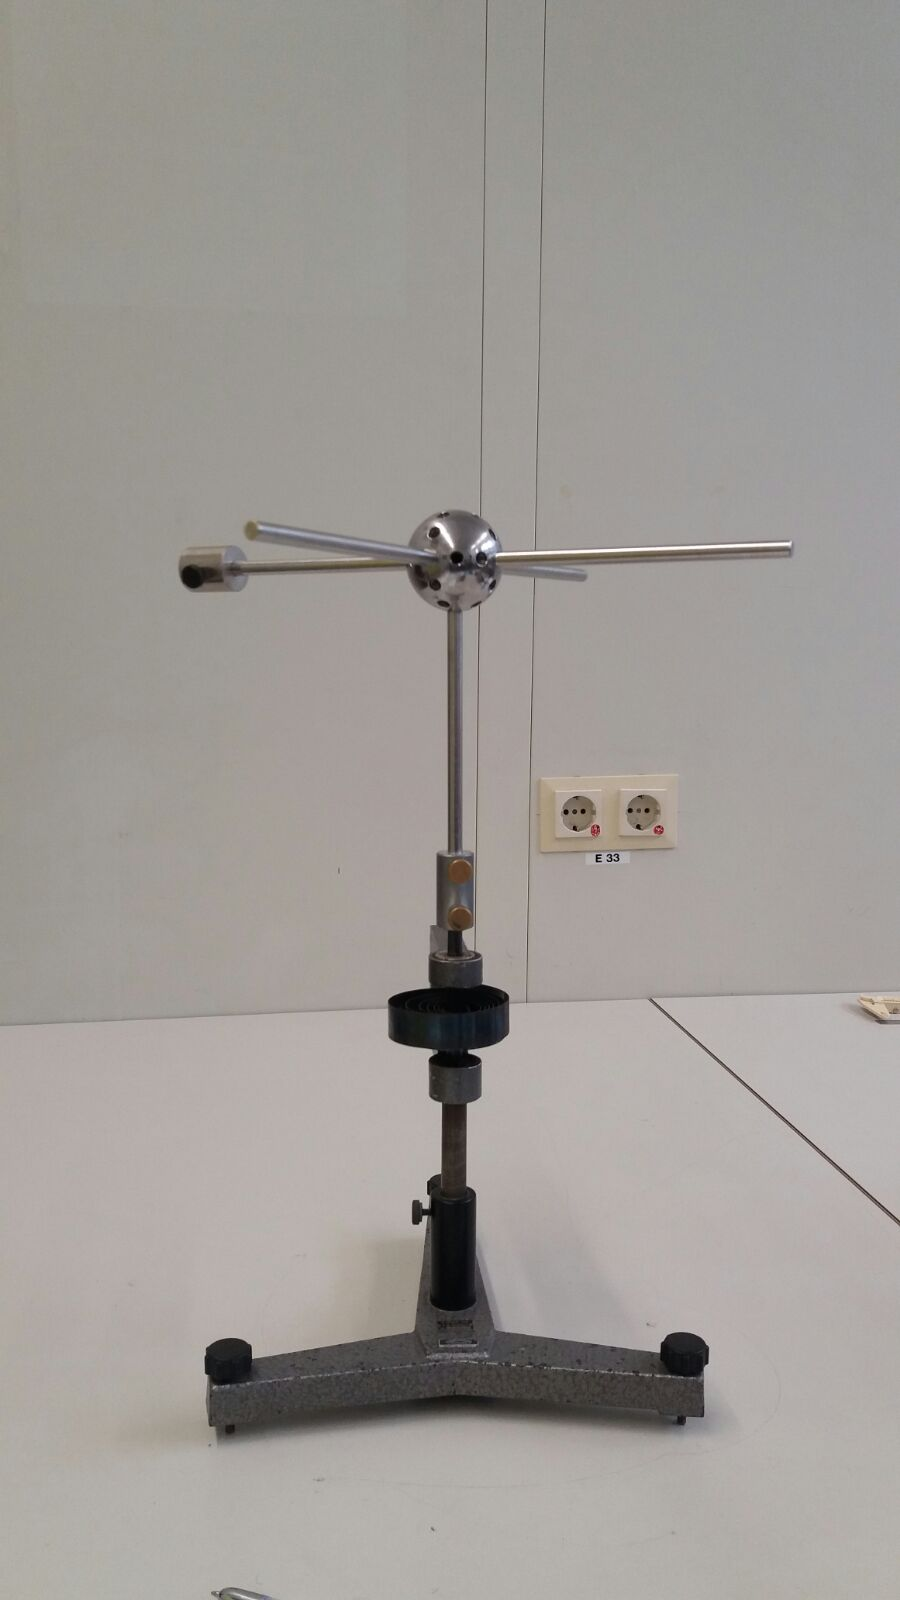
\includegraphics[scale=0.2]{aufbau.jpeg}
    \captionof{figure}[asd]{Versuchsaufbau}
    \end{center}
    
	
		In den ersten zwei Versuchsteilen soll die Winkelrichtgröße der Schneckenfeder auf zwei verschiedene Weisen bestimmt werden. Im ersten Teil wird die statische Methode zur Bestimmung genutzt. Dazu wird die nötige Kraft für eine Umdrehung von 2 $\pi$ bestimmt. Im zweiten Teil wird die dynamische Methode verwendet.  Hierfür wird die Schwingdauer unseres Systems bestimmt.\\
		Es stehen jeweils zwei kleine und zwei große Massen zur Verfügung. Die Masse der Gewichte wird durch Kraftmesser bestimmt. 
		Hierbei werden alle vier Stangen in einer Ebene eingedreht und die zwei kleinen Massen verwendet.\\
		Für die dynamische Methode lenkt man die Massen in zwei verschiedenen Abständen $l_1$ und $l_2$ vom Mittelpunkt um eine Viertel Umdrehung aus und misst daraufhin je 5 Perioden der Schwingung.\\
		Dies wird 5 mal wiederholt. \\

		\section{Versuchsteil 3a}
			Im folgenden Versuchsteil wird ein Körper konstruiert, der eine starke anisotrope Massenverteilung besitzt. Der Abstand der zwei verwendeten Massen vom Zentrum beträgt 13,5 cm. Wie in der Versuchsanleitung\footnote{Versuchsanleitung M10a, Uni Stuttgart. 2. August 2016} zu sehen, wird die Drehachse verändert. Die in Tabelle (4.3) angegebenen Buchstaben und Zahlen stehen für die jeweiligen Bezeichnungen der Bohrungen, durch diese die Drehachse geht. (Abbildung 2.2)\\
            
  \begin{center}
  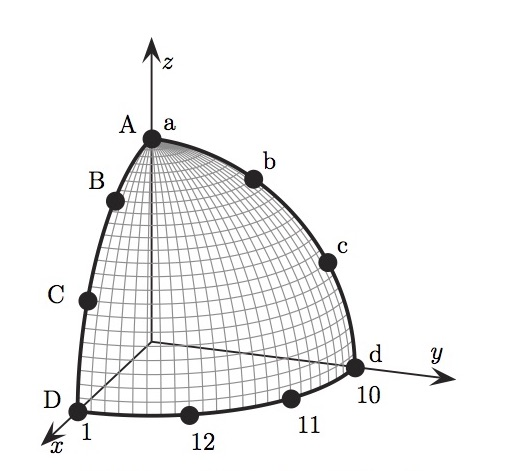
\includegraphics[scale=0.4]{1_M10.jpg}
  \captionof{figure}[asd]{Kugeloktant\protect\footnotemark}
  \footnotetext{Versuchsanleitung M10a, Uni Stuttgart. 2. August 2016}
  \end{center}
% ich bekomme das Bild aus dem Skrippt nicht rauskopiert.
		\section{Versuchsteil 3b}
			Dieselben Messungen werden Anschließend mit gleichmäßiger Massenverteilung durchgeführt. Hierfür wurden keine Gewichte an die Stangen gehängt, um möglichst nahe an einer homogenen Massenverteilung zu sein.
%----------------------------------------------------------
% Formeln
%----------------------------------------------------------
	\chapter{Formeln}
    %statistische Methode
    	Die Winkelrichtgröße D' erhält man über die Auslenkung (statische Methode) durch
        \begin{equation}
        	D' = \frac{F \cdot r}{\phi}
        \end{equation}
		Bestimmung der Winkelrichtgröße D' durch Messung der Schwingungsdauer (dynamische Methode).\\
        \begin{equation}
			D'=\frac{4\pi^2 \cdot 2m\cdot (l_1^2-l_2^2)}{(T_1^2-T_2^2)}\\
            \label{winkelrichtgroesse}
		\end{equation}
        
        ($l_1, l_2$: Abstand der Massen vom Mittelpunkt. $T_1, T_2$: Periodendauer. $m$: Masse.)
        \\
       
             Die Formel der Schwingdauer T wird durch das Trägheitsmoment J und die Winkelrichtgröße der Schneckenfeder beschrieben.
	\begin{equation}
		T = 2 \pi \sqrt{\frac{J}{D'}}
        \label{traegheitsmoment}
	\end{equation}
    ($J$: Trägheitsmoment. $D'$ Winkelrichtgröße.)\\
	\pagebreak
		
%--------------------------------------------------------
%Messwerte
%--------------------------------------------------------
		
    \chapter{Messwerte}
 Es stehen zwei Massen zur Verfügung. Auf die kleine Masse wirkt eine Gewichtskraft von 1,05 N. Bei den großen Massen wirkt eine Gewichtskraft von 2,05 N.
 \section{Bestimmung von D'}
 	\subsection{Statische Methode}
		15,6 cm vom Mittelpunkt wirkt bei $360^\circ$ eine Rückstellkraft von 0,96 N.\\
    	Messungen mit Auslenkung $\phi = \frac{\pi}{2}$ und über 5 Perioden aufgenommen. 
        \subsection{Dynamische Methode}
        \begin{multicols}{2}
			\begin{center}
				\begin{tabular}{r|l}
                	n &  $5 \cdot T_{1n}$ \\ \hline \hline
					1 & 18,09s \\ 
					2 & 17,85s \\ 
					3 & 17,85s \\ 
					4 & 17,82s \\ 
					5 & 17,85s \\ \hline 
					$\bar T_1 $ & 3,5784s
           		\end{tabular}
                \captionof{table}[l = 13,5 cm]{l = 13,5 cm}
			\end{center}
		    	
			\begin{center}
				\begin{tabular}{r|l}
					n &  $5 \cdot T_{2n}$ \\ \hline \hline						
                    1 & 11,06s \\ 
					2 & 10,97s \\ 
					3 & 11,00s \\ 
					4 & 11,00s \\ 
					5 & 11,00s \\ \hline
                    $\bar T_2 $ & 2,2012s
				\end{tabular}
                \captionof{table}[l = 4 cm]{l = 4 cm}
			\end{center}
       	\end{multicols}
		
        \section{Messungen des anisotropen und isotropen Körpers}
        
			\begin{tabular}{l|l|l|l|l|l|l|l|l|l}
   & 	   A/a & B      & C      & D/1    & 12     & 11     & d/10   & c      & b	 \\ \hline \hline
$T_1$   & 7,37   & 10,32  & 14,78  & 16,18  & 9,72   & 15,75  & 16,37  & 15,22  & 9,78   \\
$T_2$   & 7,37   & 10,28  & 14,50  & 16,25  & 9,85   & 15,91  & 16,28  & 15,16  & 9,59   \\
$T_3$   & 7,50   & 10,47  & 14,56  & 16,18  & 9,66   & 15,91  & 16,35  & 15,32  & 9,85   \\ \hline
$\bar{T}$   & 1,4827 & 2,0713 & 2,9227 & 3,2407 & 1,9487 & 3,1713 & 3,2667 & 3,0467 & 1,9480 
\end{tabular}
\captionof{table}[l = 13,5 cm]{Messungen anisotroper Körper}
\ \\
			\begin{tabular}{l|l|l|l|l|l|l|l|l|l}
				 & A/a    & B      & C      & D/1    & 12     & 11     & d/10   & c      & b      \\ \hline \hline 
				$T_1$   & 10,28  & 9,63   & 8,16   & 10,37  & 9,66   & 9,63   & 7,28   & 10,13  & 7,47   \\ 
				$T_2 $  & 10,28  & 9,53   & 8,18   & 10,33  & 9,56   & 9,63   & 7,35   & 10,12  & 7,35   \\
				$T_3 $  & 10,25  & 9,68   & 8,13   & 10,38  & 9,59   & 9,63   & 7,41   & 10,17  & 7,32   \\ \hline 
				$\bar{T}$   & 2,0540 & 1,9227 & 1,6313 & 2,0720 & 1,9207 & 1,9260 & 1,4693 & 2,0280 & 1,4760
			\end{tabular}
			\captionof{table}[l = 13,5 cm]{Messungen isotroper Körper}

        \pagebreak
        
%----------------------------------------------------------
% Formeln
%----------------------------------------------------------
        \chapter{Auswertung}
			\section{Bestimmung der Winkelrichtgröße}
				\subsubsection{über die statische Methode}
					Aus der Formel für den Drehmoment 
					\begin{equation}
						\vec{M} = D \cdot \vec{\phi}
					\end{equation}
					folgt mit 
					\begin{equation}
						\vec{M} = \vec{F} \times \vec{r}
					\end{equation}
					für die Winkelrichtgröße
            
					\begin{equation}
						D' = \frac{F \cdot r}{\phi}
					\end{equation}
           
					Aus unserer Messung ergibt sich ein Wert von
					\begin{equation}
						D' = \frac{F \cdot r}{\phi} = \frac{0,96 N \cdot 0,156m}{2 \pi} \approx 0,0238 \frac{Nm}{rad}
					\end{equation}
     
        
				\subsubsection{über die dynamische Methode}
        	
					Aus den gemessenen Zeiten werden die Mittelwerte der Perioden gebildet (siehe Abschnitt Messwerte).\\
					$\bar T_1 = 3,5784 s$\\  $\bar T_2 = 2,2012s $\\
					Mit Formel \ref{winkelrichtgroesse} ergibt sich für die Winkelrichtgröße ein Wert von
					\begin{equation}
						D'=\frac{4\pi^2\cdot 2\cdot 0,107kg\cdot ((0,135m)^2-(0,04m)^2)}{(3,5784 s)^2-(2,2012s)^2} \approx 0,0241 \frac{Nm}{rad}
					\end{equation}
					Für die weiteren Berechnungen verwenden wir den gerundeten Mittelwert aus der dynamischen und der statischen Methode $\bar D = 0,024 \frac{Nm}{rad}$.
        \pagebreak
        
		\section{Trägheitsellipsoid eines anisotropen Körpers}
				Aus der Symmetrie des Körpers ergeben sich die Hauptträgheitsachsen 
				\begin{center}
            \begin{tabular}{r|l}
					Bohrung &  Trägheitsmoment \\ \hline \hline
					A/a & $J_{z}$ \\ 
					D/1 & $J_{y}$ \\ 
					d/10 & $J_{x}$ 
				\end{tabular}
			\end{center}
            Für das Trägheitsmoment gilt mit Formel \ref{traegheitsmoment}
            \begin{equation}
            	J_{x} = \frac{T_{x}^2 \cdot D'}{4\pi^2} = \frac{(3,24s)^2 \cdot 0,024 \frac{Nm}{rad}}{4\pi^2} =  6,4\cdot10^{-3} \frac{kgm^2}{rad} 
            \end{equation}
            \begin{equation}
            	J_{y} = 6,5\cdot10^{-3} \frac{kgm^2}{rad} 
            \end{equation}
            \begin{equation}
            	J_{z} = 1,3\cdot10^{-3} \frac{kgm^2}{rad} 
            \end{equation}
            
            
        \section{Trägheitsellipsoid eines isotropen Körpers}
        
            \begin{equation}
            	J_{x} = \frac{T_{x}^2 \cdot D'}{4\pi^2} = \frac{(2,07s)^2 \cdot 0,024 \frac{Nm}{rad}}{4\pi^2} = 2,6 \cdot 10^{-3}\frac{kgm^2}{rad} 
            \end{equation}
            \begin{equation}
            	J_{y} = 1,3 \cdot 10^{-3}\frac{kgm^2}{rad}
            \end{equation}
            \begin{equation}
            	J_{z} = 2,6 \cdot 10^{-3}\frac{kgm^2}{rad}
            \end{equation}
            
            \section{Plot des Kugeloktanden}
           Um die Trägheitsmomente zu plotten können wir die zu $\frac{1}{\sqrt[]{J}}$ proportionale und leichter zu berechnende Größe $\frac{1}{T}$ verwenden.\\
            \begin{tabular}{l|lllllllll}
anisotrop &A/a & B      & C      & D/1    & 12     & 11     & d/10   & c      & b       \\\hline
$\frac{1}{T} ~ [\frac{1}{s}]$ & 0,6745 & 0,4828 & 0,3422 & 0,3086 & 0,5132 & 0,3153 & 0,3061 & 0,3282 & 0,5133 \\ \hline \hline
Isotrop & A/a    & B      & C      & D/1    & 12     & 11     & d/10   & c      & b      \\ \hline
$\frac{1}{T} ~ [\frac{1}{s}]$& 0,4869 & 0,5201 & 0,6130 & 0,4826 & 0,5207 & 0,5192 & 0,6806 & 0,4931 & 0,6775
\end{tabular}
	\captionof{table}[]{Daten für den Plot des Kugeloktanten}
 				\begin{gnuplot}[terminal=pdf,terminaloptions={font ",10" linewidth 3},scale=1.2]      
   				unset border
set polar
set angles degrees #set gnuplot on degrees instead of radians

set style line 10 lt 1 lc 0 lw 0.3 #redefine a new line style for the grid

set grid polar 30 #set the grid to be displayed every 60 degrees
set grid ls 10

set xrange [-0.8:0.8] #make gnuplot to go until 6000
set yrange [-0.8:0.8]

set xtics axis #disply the xtics on the axis instead of on the border
set ytics axis

set xtics scale 0 #"remove" the tics so that only the y tics are displayed
set xtics ("" 1000, "" 2000, "" 3000, "" 4000, "" 5000, "" 6000) #set the xtics only go from 0 to 6000 with increment of1000 but do not display anything. This has to be done otherwise the grid will not be displayed correctly.
set ytics 0, 1000, 6000 #make the ytics go from the center (0) to 6000 with incrment of 1000

set size square 

set key lmargin

set_label(x, text) = sprintf("set label '%s' at (0.9*cos(%f)), (0.9*sin(%f))     center", text, x, x) #this places a label on the outside

#here all labels are created
eval set_label(0, "A/a")
eval set_label(30, "B")
eval set_label(60, "C")
eval set_label(85, "D/1")
eval set_label(120, "12")
eval set_label(150, "11")
eval set_label(180, "d/10")
eval set_label(210, "c")
eval set_label(240, "b")
eval set_label(270, "A/a")

set style line 11 lt 1 lw 2 pt 2 ps 2 #set the line style for the plot
plot "-" using 1:2 title "isotrop" with lp, "-" using 1:3 title "anisotrop" with lp
0	0.4869	0.6745
30	0.5201	0.4828
60	0.6130	0.3422
90	0.4826	0.3086
120	0.5207	0.5132
150	0.5192	0.3153
180	0.6806	0.3061
210	0.4931	0.3282
240	0.6775	0.5133
270	0.4869	0.6745
e
0	0.3061	0.6745
30	0.5201	0.4828
60	0.6130	0.3422
90	0.3282	0.3086
120	0.5206	0.5132
150	0.5192	0.3153
180	0.6805	0.3061
210	0.3421	0.3282
240	0.6775	0.5133
270	0.3061	0.6745
e
\end{gnuplot}
    \captionof{figure}[]{Plot von $\frac{1}{T}$ auf dem Kugeloktanten}
%----------------------------------------------------------
% Formeln
%----------------------------------------------------------
           \chapter{Fehlerrechnung}
           \section{Betrachtung der Fehlerquellen}
           Es kann an folgenden Stellen zu Messfehlern gekommen sein.
           
\begin{itemize}
\item Beim Ablesen vom Lineal
\item Beim Stoppen der Zeit aufgrund von Reaktionszeit und Unsicherheit beim eintreten des Umkehrpunkts
\item Bei der Bestimmung der Masse
\end{itemize}

Da die Masse über einen Kraftmesser mit einer Skalenauflösung von 0,2 Newton gemessen wurde, kann man einen Fehler von 
 \begin{equation}
 \Delta m = \frac{\Delta F}{g} = \frac{0,2 N}{9,81 \frac{m}{s^2}} \approx 0,02 \si{\kilo\gram} 
 \end{equation}
 annehmen.
\\
Das verwendete Lineal hat eine Skalenauflösung von $0,001m$, also kann man einen Fehler von 
\begin{equation}
	\Delta l = 10^{-3} m
\end{equation}
erwarten.
\\
Um den Fehler der Zeitmessung zu reduzieren, wurde je über 5 Perioden gemessen. Gehen wir davon aus, dass durch Reaktionszeit und ungenaues Erkennen des Umkehrpunkts ein Fehler von $0,5s$ auftritt, dann sind das $0,1s$ pro Periode und damit
\begin{equation}
	\Delta t = 0,1s
\end{equation}
Außerdem konnte es bei der Auslenkung der Feder zu Fehlern gekommen sein.
\begin{equation}
    		\Delta \phi = 2^\circ \hat{=} \frac{1}{90}\pi
    	\end{equation}
	\section{Fehler für D' in der statischen Methode über die Fehlerfortpflanzung}
    	\begin{equation}
    		D' = \frac{F \cdot r}{\phi}
    	\end{equation}
        \begin{equation}
    		\Delta D' = |\frac{r}{\phi}| \Delta F + |\frac{F}{\phi}| \Delta r + |-\frac{F \cdot r}{\phi^2}| \Delta \phi
    	\end{equation}
        \begin{equation}
    		\Delta D' = |\frac{0,156m}{2\pi}| 0,2 N + |\frac{0,96N}{2\pi}| 10^{-3} m + |-\frac{0,96N \cdot 0,156m}{4\pi^2}| \frac{1}{90}\pi = 5\cdot 10^{-3} \frac{Nm}{rad}
    	\end{equation}
	\section{Fehler für D' in der dynamischen Methode über die Fehlerfortpflanzung}
    	\begin{equation}
    		D' = \frac{4\pi^2 \cdot 2m \cdot (l_1^2 - l_2^2)}{T_1^2 - T_2^2}
    	\end{equation}
     
    \begin{equation}
    \Delta D' = 
    |\frac{\delta D'}{\delta m}| \Delta m +
    |\frac{\delta D'}{\delta T_1}| \Delta T_1 +
    |\frac{\delta D'}{\delta T_2}| \Delta T_2 + 
    |\frac{\delta D'}{\delta l_1}| \Delta l_1 + 
    |\frac{\delta D'}{\delta l_2}| \Delta l_2
    \end{equation}
    \begin{equation}
    \begin{aligned}
    \Delta D' = 
    |\frac{4\pi^2 \cdot 2 \cdot (l_1^2 - l_2^2)}{T_1^2 - T_2^2}| \Delta m + 
    |\frac{2 T_1 \cdot 4\pi^2 \cdot 2m \cdot (l_1^2 - l_2^2)}{(T_1^2 - T_2^2)^2}| \Delta T_1  \\ +
    |- \frac{2 T_2 \cdot 4\pi^2 \cdot 2m \cdot (l_1^2 - l_2^2)}{(T_1^2 - T_2^2)^2}| \Delta T_2 +  
    |\frac{8\pi^2 \cdot 2m \cdot l_1}{T_1^2 - T_2^2}| \Delta l_1 \\ +
    |- \frac{8\pi^2 \cdot 2m \cdot l_2}{T_1^2 - T_2^2}| \Delta l_2
    \end{aligned}    
    \end{equation}    
    $
    \Delta D' = 
    |\frac{4\pi^2 \cdot 2 \cdot ((0,135m)^2 - (0,04m)^2)}{(3,5784s)^2 - (2,2012s)^2}| 0,02kg + \\
    |\frac{2  (3,5784s) \cdot 4\pi^2 \cdot 2 (0,107kg) \cdot ((0,135m)^2 - (0,04m)^2)}{((3,5784s)^2 - (2,2012s)^2)^2}| 0,1s +
    |- \frac{2 (2,2012s) \cdot 4\pi^2 \cdot 2 (0,107kg) \cdot ((0,135m)^2 - (0,04m)^2)}{((3,5784s)^2 - (2,2012s)^2)^2}| 0,1s + 
    |\frac{8\pi^2 \cdot 2 (0,107kg)  \cdot (0,135m)}{(3,5784s)^2 - (2,2012s)^2}| 0,001m + 
    |- \frac{8\pi^2 \cdot 2 (0,107kg)  \cdot (0,04m)}{(3,5784s)^2 - (2,2012s)^2}| 0,001m = 8,4\cdot 10^{-3} \frac{Nm}{rad}
    $
   
\section{Fehler für J über die Fehlerfortpflanzung}
    \begin{equation}
    J = \frac{T^2 \cdot D'}{4 \pi^2}
     \end{equation}
    
    \begin{equation}
    \Delta J = 
    |\frac{2 T \cdot D'}{4 \pi^2}| \Delta T +
    |\frac{T^2}{4 \pi^2}| \Delta D'
     \end{equation}
    \begin{equation}
    \Delta J_x = 
    |\frac{2 (3,2407s) \cdot (0,024 \frac{Nm}{rad})}{4 \pi^2}| 0,1s +
    |\frac{(3,2407s)^2}{4 \pi^2}| 0,008\frac{Nm}{rad} \approx 2,5 \cdot 10^{-3} \frac{kgm^2}{rad}
     \end{equation}
   
   Analog für die restlichen Werte siehe Tabelle 6.1 \\
   
   \begin{center}
   \begin{tabular}{l|c|c}
			&	Anisotrop  & Isotrop    \\ \hline \hline
		$\Delta J_x [\frac{kgm^2}{rad}]$ & $2,5 \cdot 10^{-3}$ & $1,2 \cdot 10^{-3}$ \\
		$\Delta J_y [\frac{kgm^2}{rad}]$ & $2,7 \cdot 10^{-3}$ & $0,6 \cdot 10^{-3}$ \\
		$\Delta J_z [\frac{kgm^2}{rad}]$ & $0,7 \cdot 10^{-3}$ & $1,6 \cdot 10^{-3}$
	\end{tabular}
    \captionof{table}[Hauptt]{Fehler der Hauptträgheitsmomente}
   	\end{center}
   
   \pagebreak
%----------------------------------------------------------

%----------------------------------------------------------
	\chapter{Zusammenfassung}
    	In diesem Versuch wurde von einem Kreisel das Trägheitsmoment bestimmt. Die bestimmten Werte mit Fehler lauten: \\
        \begin{center}
        
   	\begin{tabular}{l|c|c}
			&	Anisotrop  & Isotrop    \\ \hline \hline
		$J_x [\frac{kgm^2}{rad}]$ & $(6,4 \pm 2,5) \cdot 10^{-3}$& $(2,6 \pm 1,2) \cdot 10^{-3}$ \\
		$J_y [\frac{kgm^2}{rad}]$ & $(6,5 \pm 2,7) \cdot 10^{-3}$ & $(1,3 \pm 0,6) \cdot 10^{-3}$ \\
		$J_z [\frac{kgm^2}{rad}]$ & $(1,3 \pm 0,7) \cdot 10^{-3}$ & $(2,6 \pm 1,6) \cdot 10^{-3}$
	\end{tabular}
    	\captionof{table}[]{Trägheitsmomente auf den Hauptträgheitsachsen mit Fehler}
    
        \end{center}
      	Als Winkelrichtgröße wurde der Wert	$(24 \pm 8) \cdot 10^{-3} \frac{Nm}{rad}$
        als gemittelter Wert der statischen und dynamischen Methode bestimmt. \\
     	Gründe für den Fehler sind:
     	\begin{itemize}
       		\item Ungenauigkeit bei der Bestimmung der Massen. Hierbei wurden die Massen über ungenaue Kraftmesser bestimmt.
        	\item Ungenauigkeit beim Stoppen der Zeit.
        	\item Ungenauigkeit beim bestimmen vom Abstand der Massen zum Mittelpunkt.
        	\item Keine exakte Massenverteilung.
      	\end{itemize}
	\pagebreak
%----------------------------------------------------------

%----------------------------------------------------------
    \chapter{Anhang}
    	\begin{center}
    		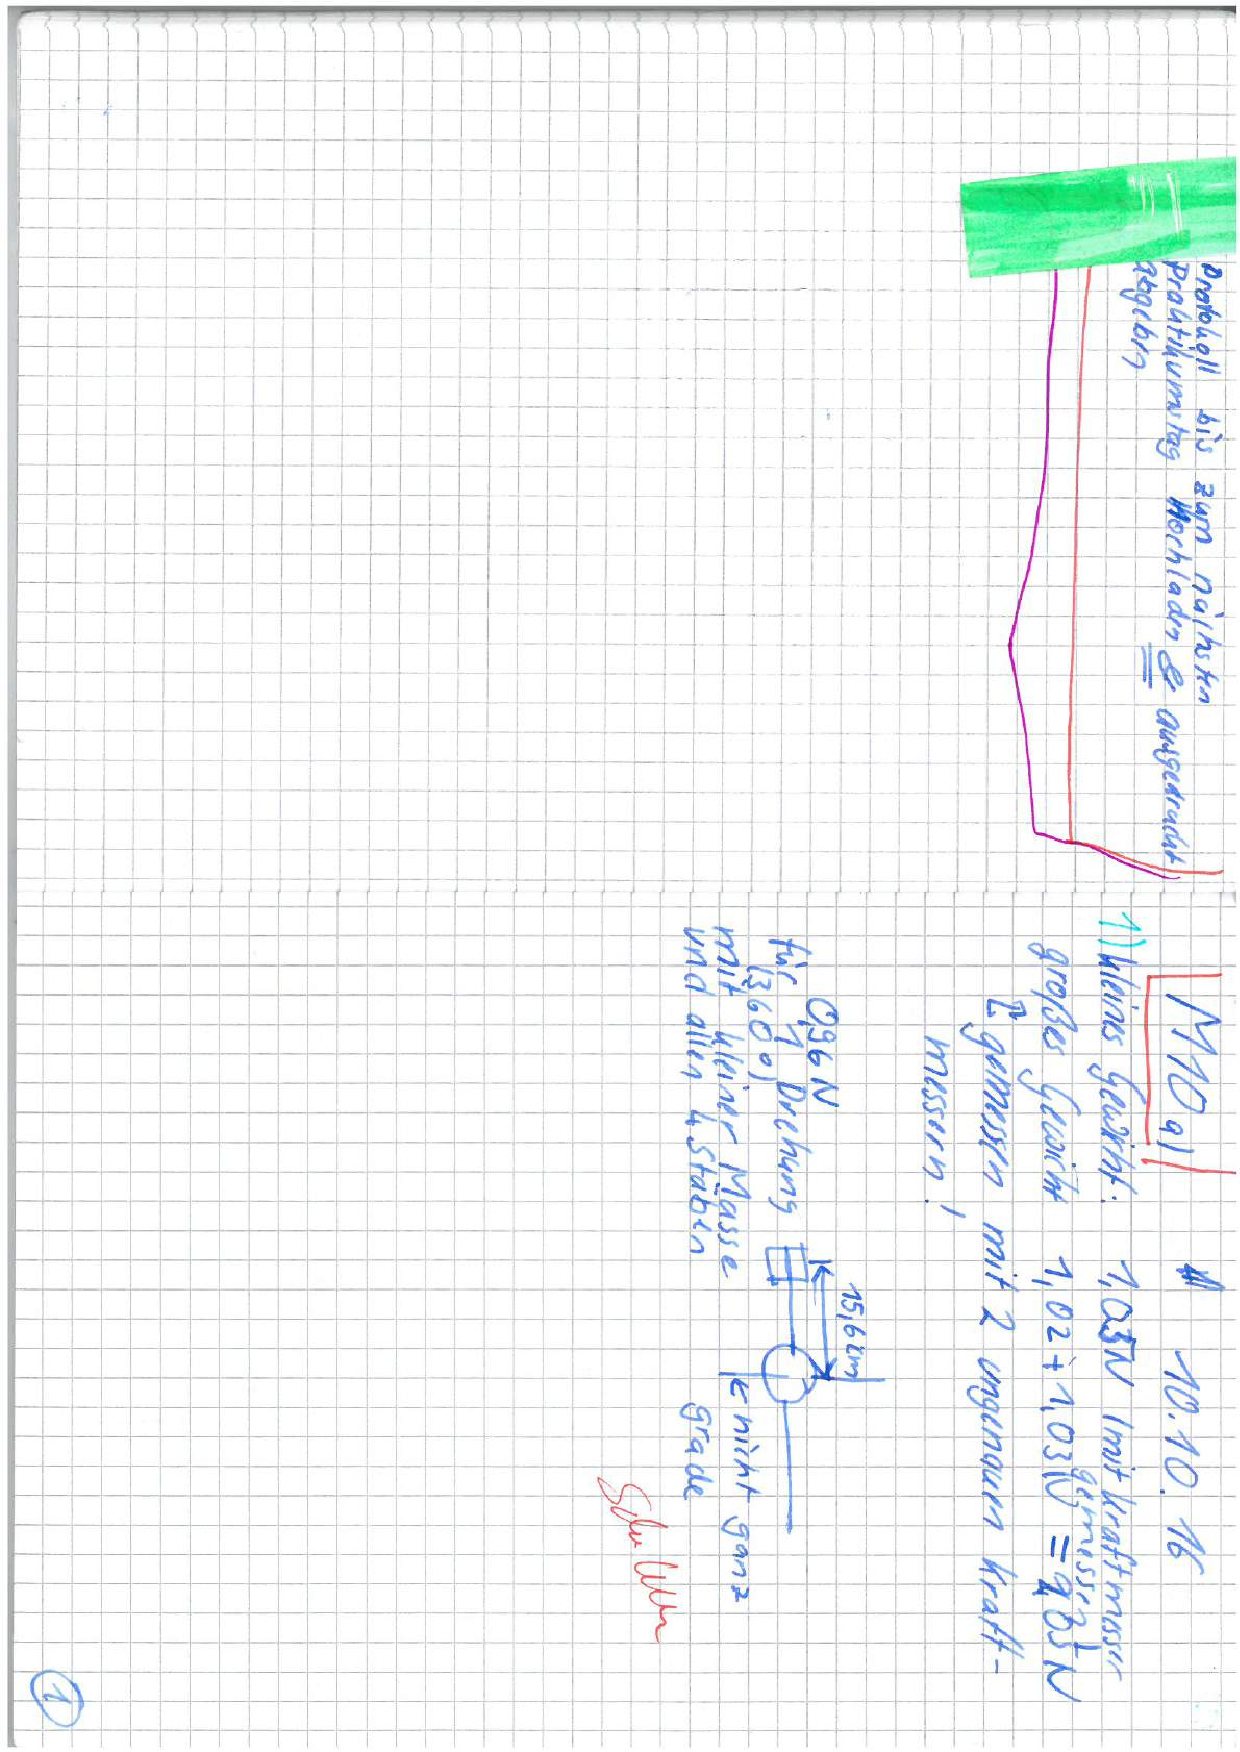
\includegraphics[scale=0.65]{1.pdf}
    	\end{center}
    	\captionof{figure}[Seite 1]{Messprotokoll Seite 1}
    	\pagebreak
    	
        \begin{center}
    		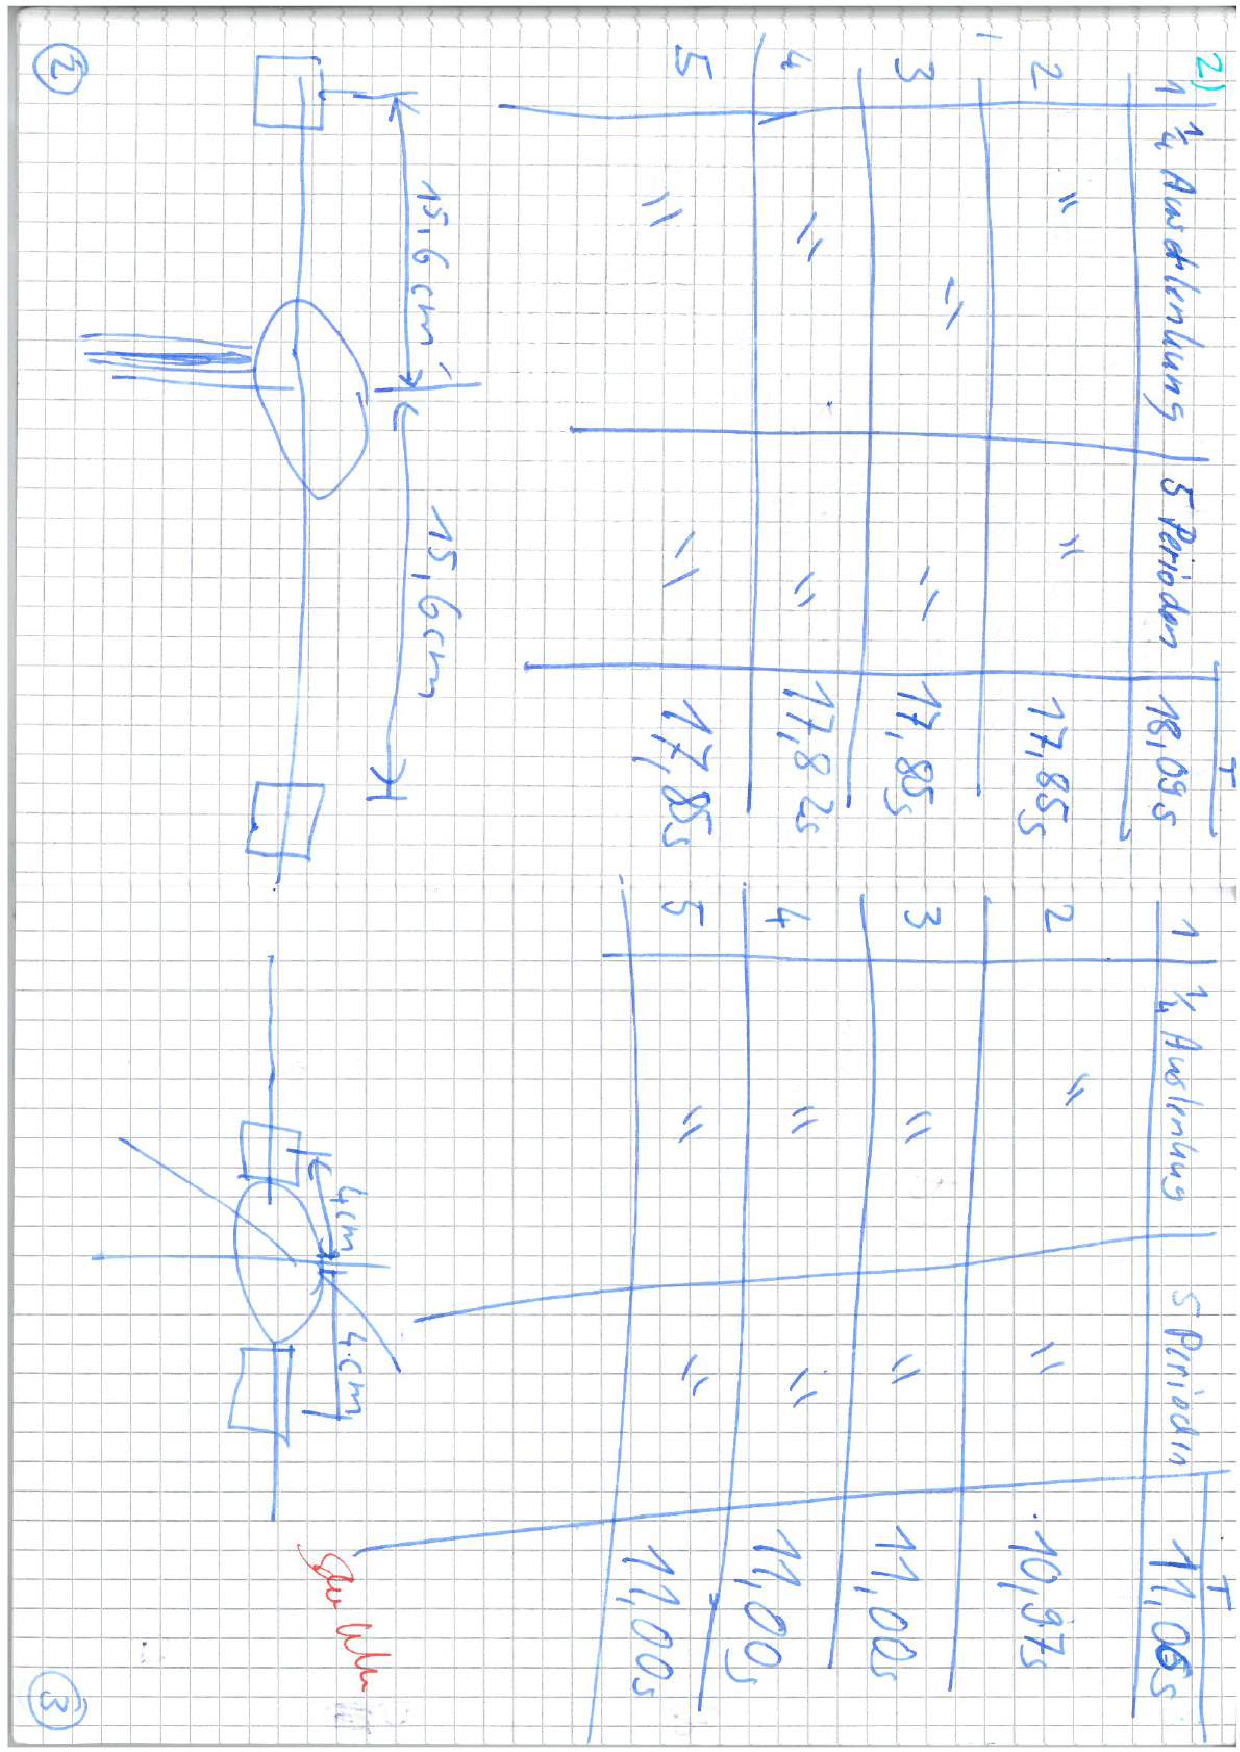
\includegraphics[scale=0.7]{2.pdf}
    	\end{center}
    	\captionof{figure}[Seite 2]{Messprotokoll Seite 2}
    	\pagebreak
    	
        \begin{center}
   		 	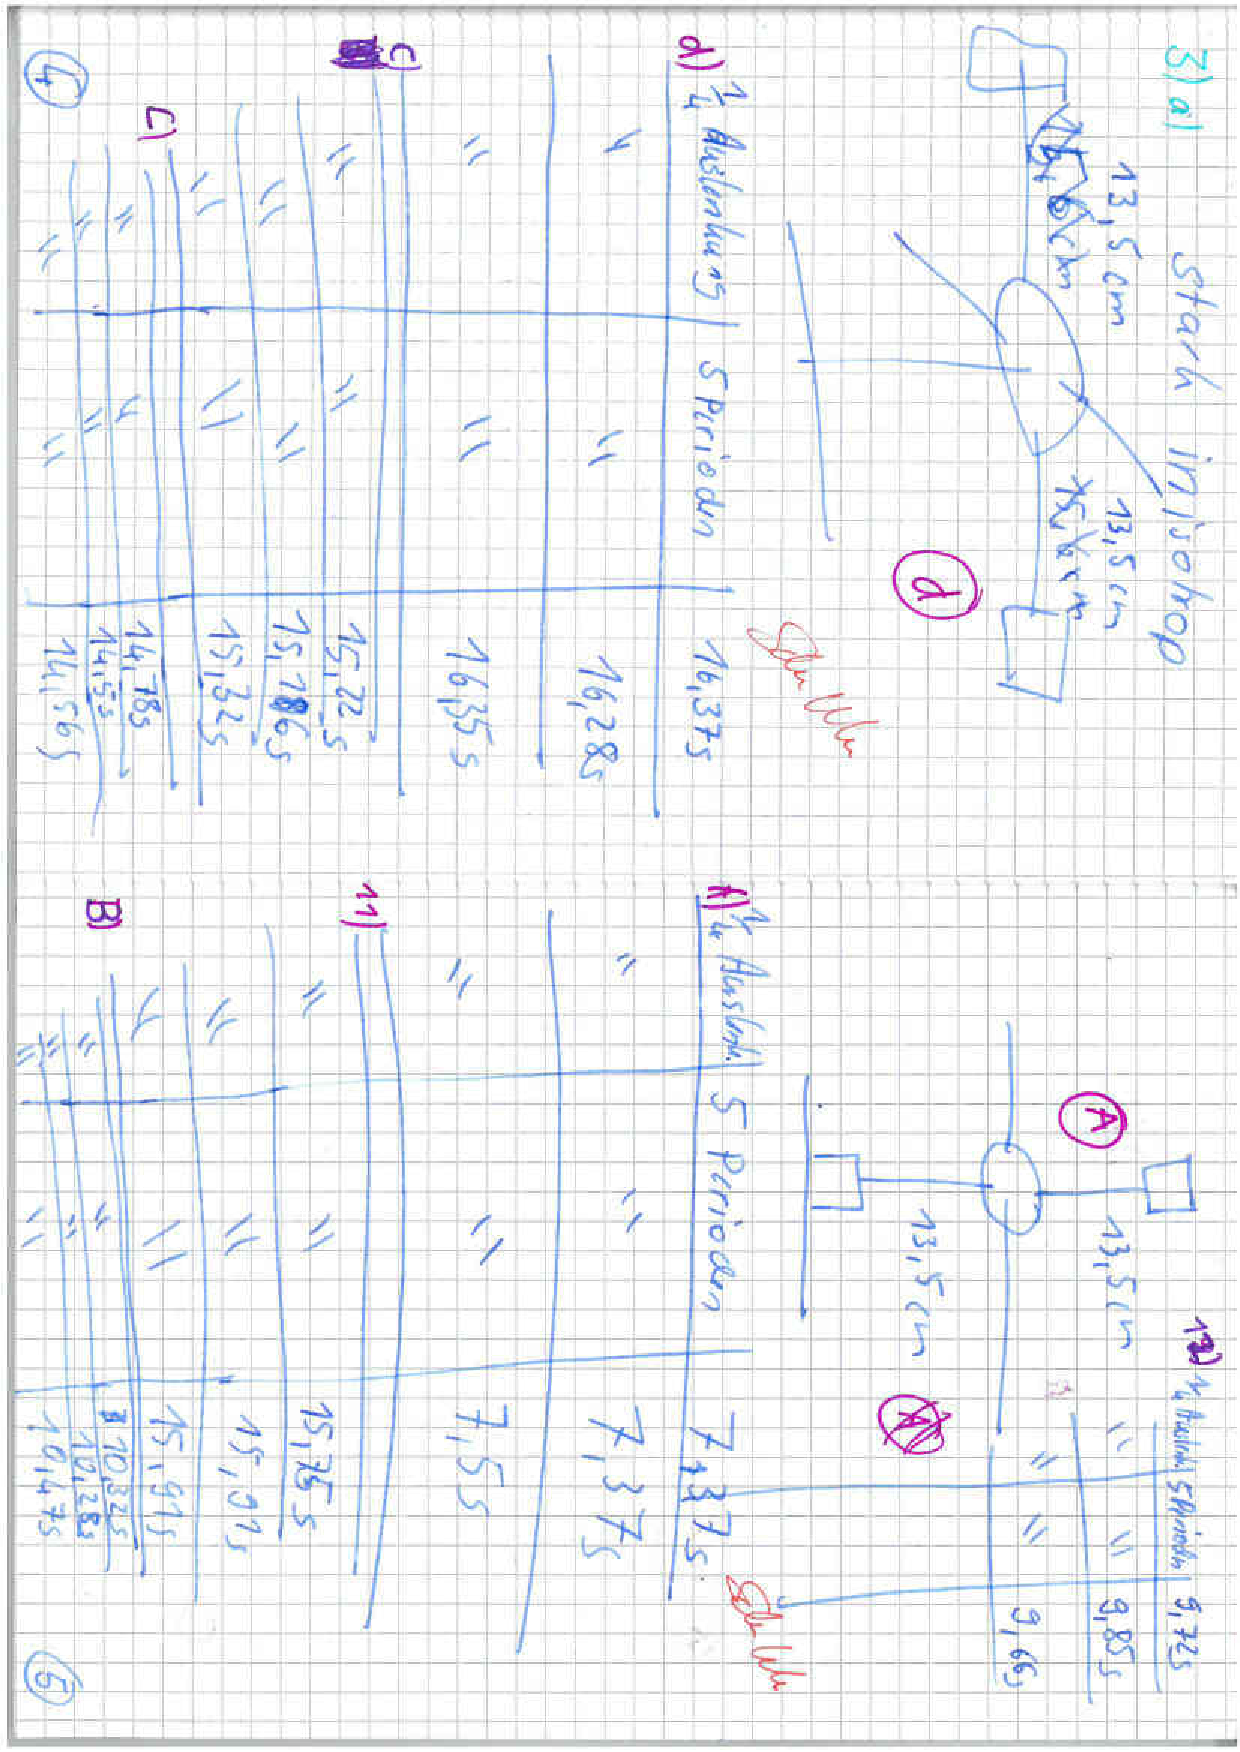
\includegraphics[scale=0.7]{3.pdf}
   	 	\end{center}
    	\captionof{figure}[Seite 3]{Messprotokoll Seite 3}
    	\pagebreak
    	
        \begin{center}
    		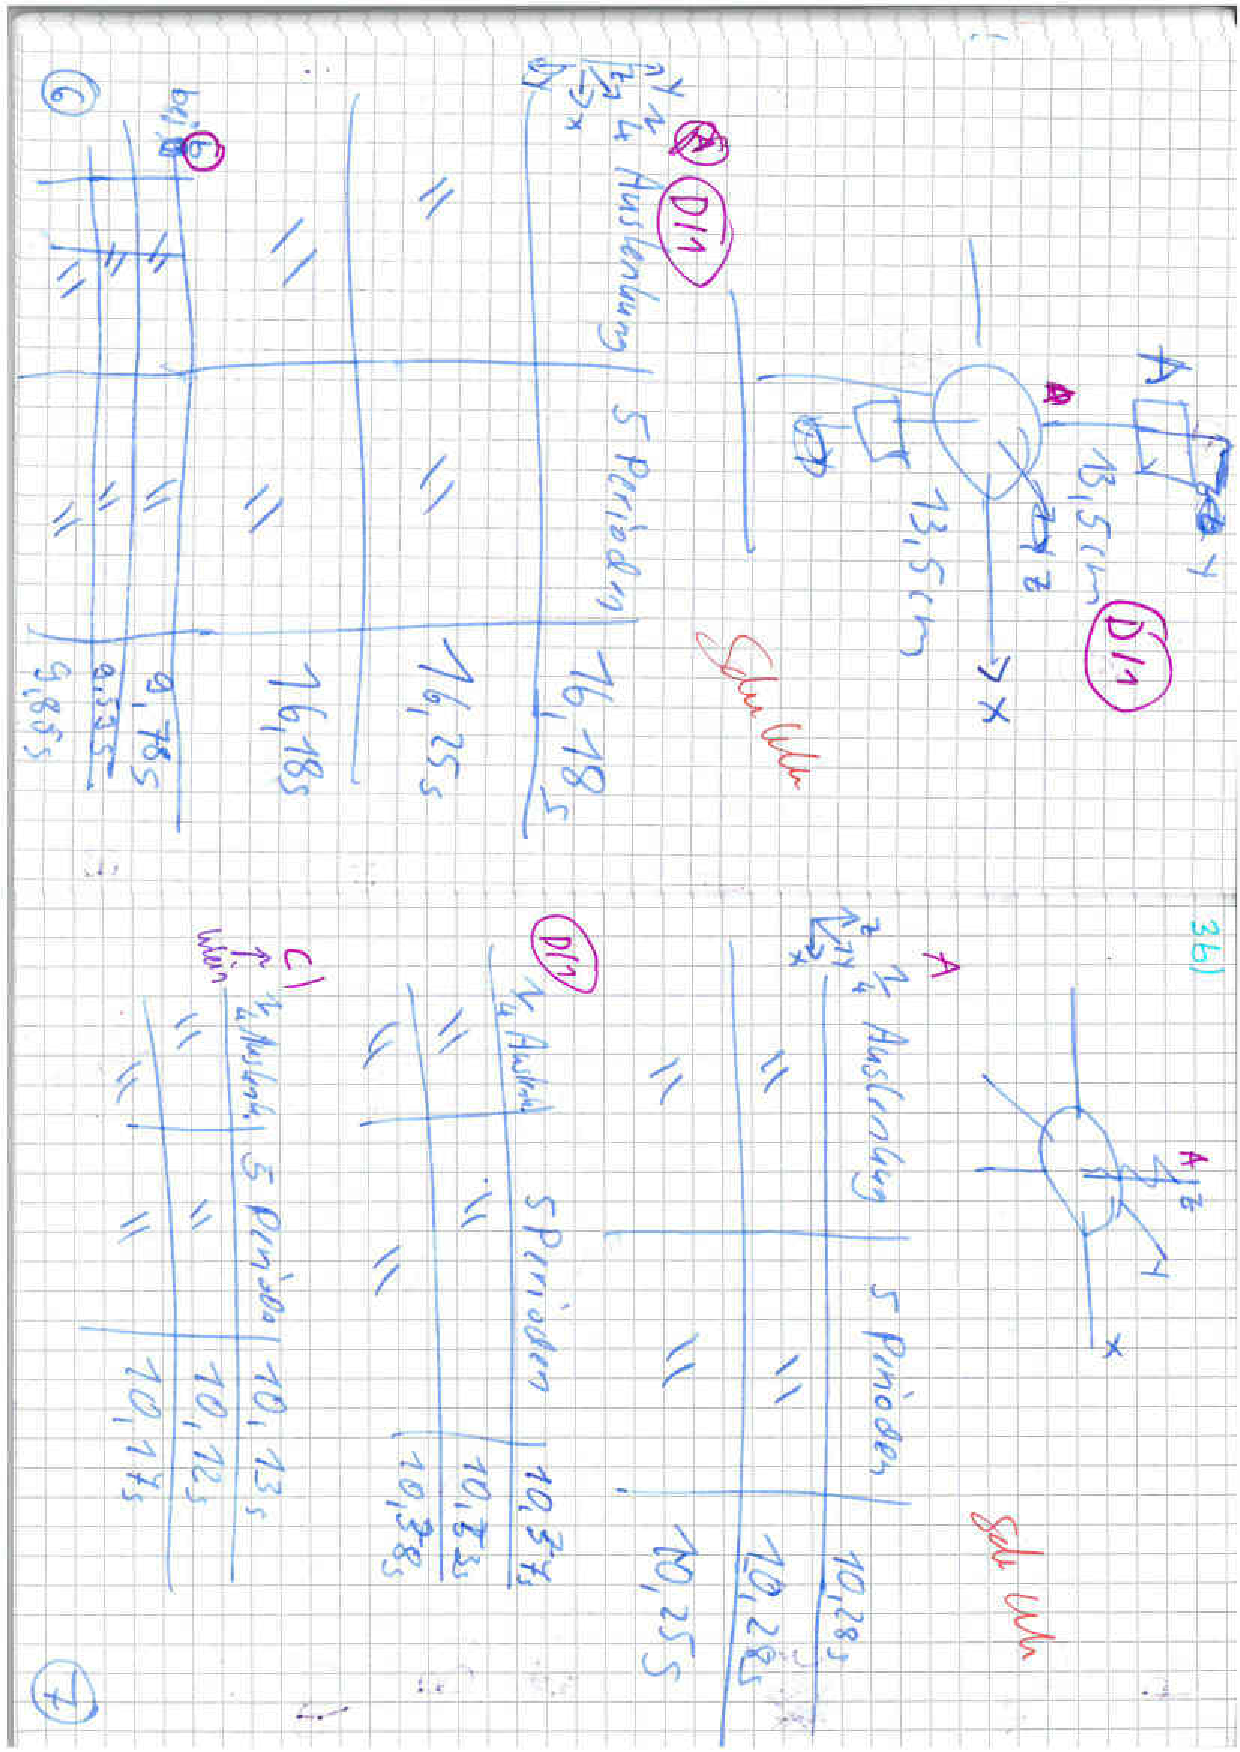
\includegraphics[scale=0.7]{4.pdf}
    	\end{center}
    	\captionof{figure}[Seite 4]{Messprotokoll Seite 4}
    	\pagebreak
    	
        \begin{center}
    		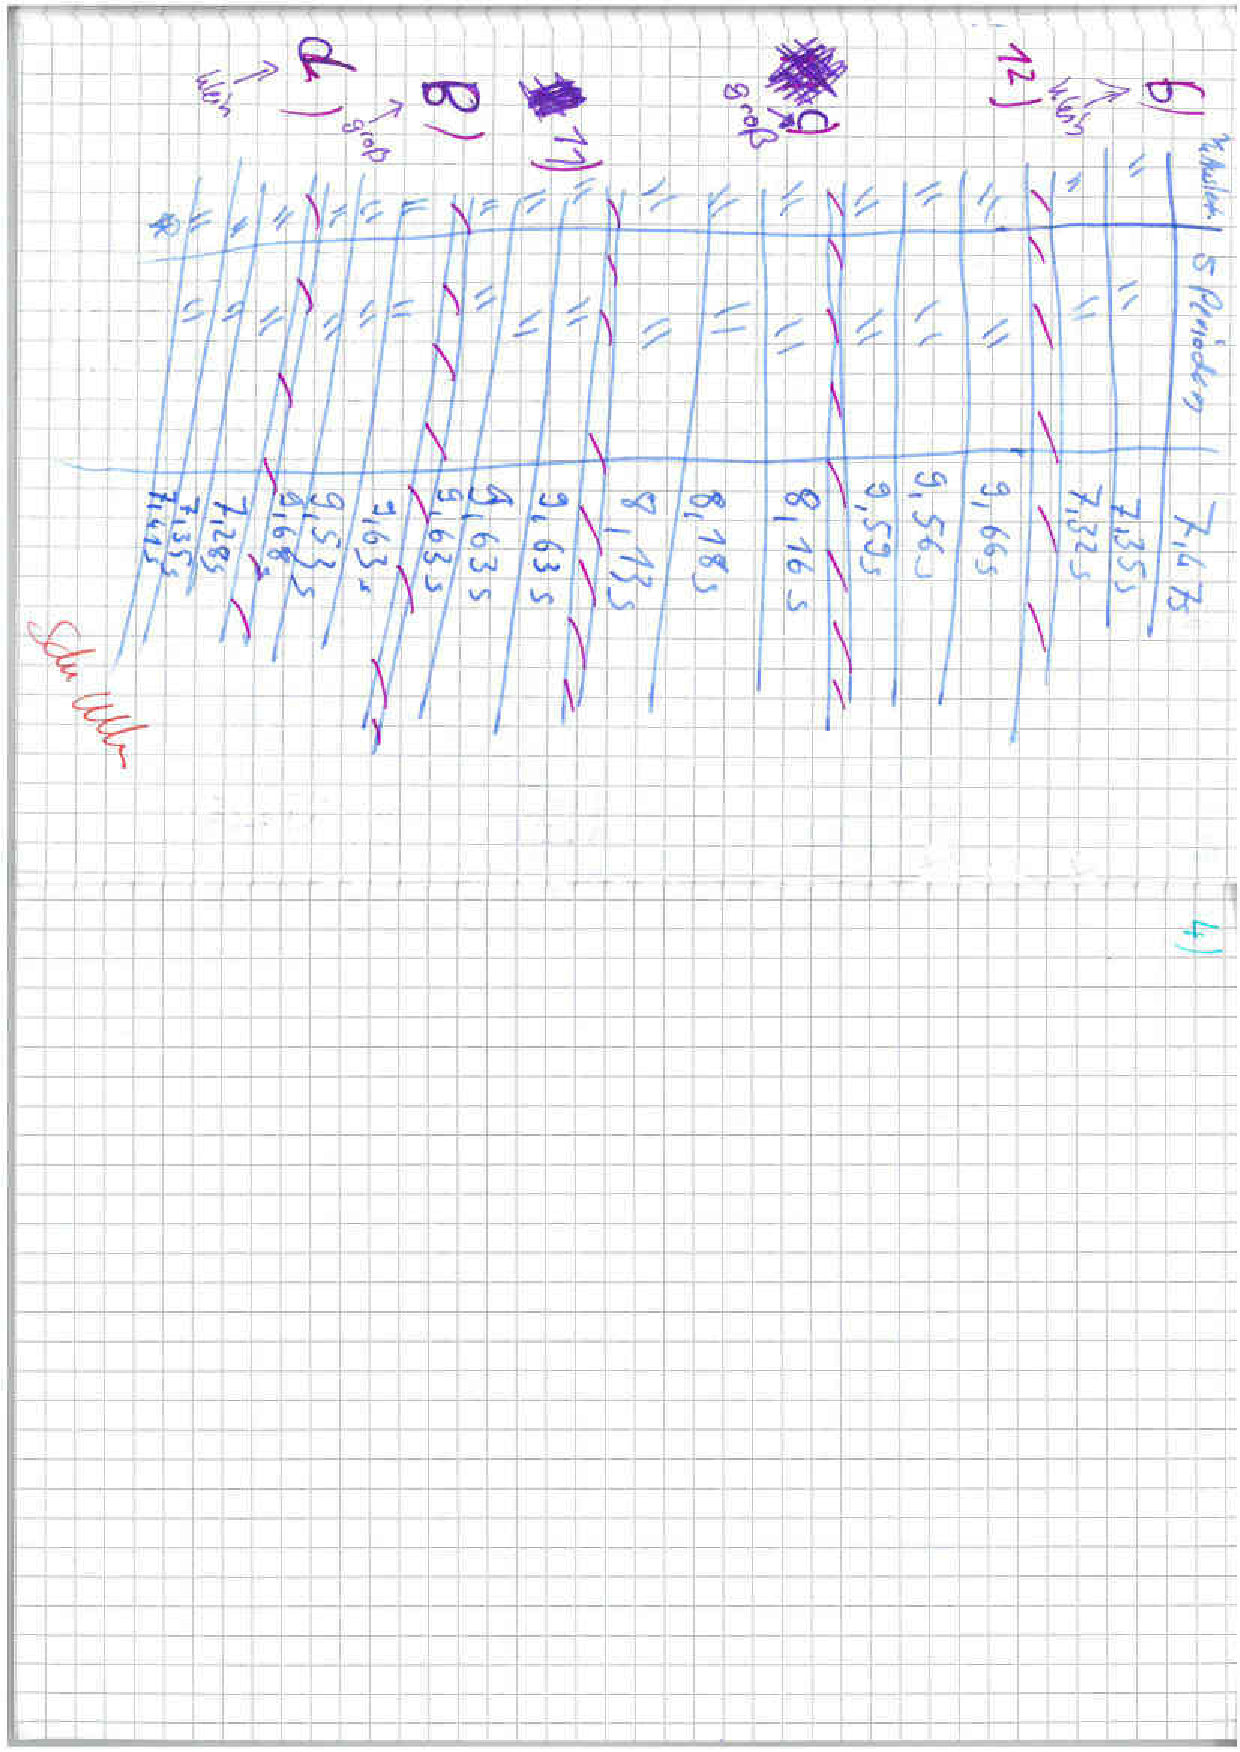
\includegraphics[scale=0.7]{5.pdf}
    	\end{center}
    	\captionof{figure}[Seite 5]{Messprotokoll Seite 5}
    	\pagebreak
\end{document}
